\documentclass[10pt]{article} 

%\usepackage{aistats2017}

% If your paper is accepted, change the options for the package
% aistats2017 as follows:
%
\usepackage{aistats2017}
%
% This option will print headings for the title of your paper and
% headings for the authors names, plus a copyright note at the end of
% the first column of the first page.


\usepackage{algorithm}
%\usepackage{algorithmic}
\usepackage{multirow}
\usepackage{booktabs}
\usepackage{pifont} % \checkmark
\usepackage[utf8]{inputenc} % allow utf-8 input
\usepackage[T1]{fontenc}    % use 8-bit T1 fonts
\usepackage{hyperref}       % hyperlinks
\usepackage{url}            % simple URL typesetting
\usepackage{booktabs}       % professional-quality tables
\usepackage{amsfonts}       % blackboard math symbols
\usepackage{nicefrac}       % compact symbols for 1/2, etc.
\usepackage{microtype}      % microtypography
%\usepackage[english]{babel}
%\usepackage{cite}
%\usepackage{verbatim}
\usepackage{amsmath,amsthm}
\usepackage{amssymb,amsbsy,epsfig,float}
\usepackage{graphicx,wrapfig,lipsum}
%\usepackage{graphicx}
%\usepackage{multirow}
%\usepackage{algorithmicx}
%\usepackage[ruled]{algorithm}
\usepackage{algpseudocode}
\usepackage{subfigure} 
\usepackage[makeroom]{cancel}
\usepackage{xspace}
\usepackage{mathtools}
\usepackage{bbm}

\usepackage{color}
\usepackage[usenames,dvipsnames]{xcolor}

%\usepackage[backgroundcolor = White,textwidth=\marginparwidth]{todonotes}
% To remove todo notes, simply uncomment the following line and comment out the previous one
 \usepackage[disable,backgroundcolor = White,textwidth=\marginparwidth]{todonotes}

% Comments by Csaba:
\newcommand{\todoc}[2][]{\todo[color=Apricot!20,size=\tiny,#1]{Cs: #2}}
% Comments by Manjesh:
\newcommand{\todom}[2][]{\todo[color=Cerulean!20,size=\tiny,#1]{M: #2}}
% Comments by Venkatesh:
\newcommand{\todov}[2][]{\todo[color=Purple!20,size=\tiny,#1]{V: #2}}

\newcommand{\hY}{\hat{Y}}
\newcommand{\N}{\mathbb{N}}
\newcommand{\htheta}{\hat{\theta}}
\newcommand{\iset}[1]{[#1]}
\DeclareMathOperator{\argmin}{argmin}
\newcommand{\ip}[1]{\langle #1 \rangle} % inner product
\newcommand{\SA}{\mathrm{SA}}
\newcommand{\SD}{\mathrm{SD}}
\newcommand{\WD}{\mathrm{WD}}
\newcommand{\TSA}{\Theta_{\SA}}
\newcommand{\Alg}{\mathfrak{A}}
\newcommand{\TSD}{\Theta_{\SD}}
\newcommand{\TWD}{\Theta_{\WD}}
\newcommand{\awd}{a_{\mathrm{wd}}}
\def\ddefloop#1{\ifx\ddefloop#1\else\ddef{#1}\expandafter\ddefloop\fi}

% \bA, \bB, ...
\def\ddef#1{\expandafter\def\csname b#1\endcsname{\ensuremath{\mathbf{#1}}}}
\ddefloop ABCDEFGHIJKLMNOPQRSTUVWXYZ\ddefloop

% \bbA, \bbB, ...
\def\ddef#1{\expandafter\def\csname bb#1\endcsname{\ensuremath{\mathbb{#1}}}}
\ddefloop ABCDEFGHIJKLMNOPQRSTUVWXYZ\ddefloop

% \cA, \cB, ...
\def\ddef#1{\expandafter\def\csname c#1\endcsname{\ensuremath{\mathcal{#1}}}}
\ddefloop ABCDEFGHIJKLMNOPQRSTUVWXYZ\ddefloop

% \vA, \vB, ..., \va, \vb, ...
\def\ddef#1{\expandafter\def\csname v#1\endcsname{\ensuremath{\boldsymbol{#1}}}}
\ddefloop ABCDEFGHIJKLMNOPQRSTUVWXYZabcdefghijklmnopqrstuvwxyz\ddefloop

% \valpha, \vbeta, ...,  \vGamma, \vDelta, ...,
\def\ddef#1{\expandafter\def\csname v#1\endcsname{\ensuremath{\boldsymbol{\csname #1\endcsname}}}}
\ddefloop {alpha}{beta}{gamma}{delta}{epsilon}{varepsilon}{zeta}{eta}{theta}{vartheta}{iota}{kappa}{lambda}{mu}{nu}{xi}{pi}{varpi}{rho}{varrho}{sigma}{varsigma}{tau}{upsilon}{phi}{varphi}{chi}{psi}{omega}{Gamma}{Delta}{Theta}{Lambda}{Xi}{Pi}{Sigma}{varSigma}{Upsilon}{Phi}{Psi}{Omega}\ddefloop

\newcommand{\Y}{\mathcal{Y}}
\newcommand{\A}{\mathcal{A}}
\newcommand{\EE}[1]{\mathbb{E}\left[#1\right]}
\newcommand{\EEi}[2]{\mathbb{E}_{#1}\left[#2\right]}
\newcommand{\Prob}[1]{\mathbb{P}\left(#1\right)}
\newcommand{\Regret}{\mathfrak{R}}
\newcommand{\R}{\mathbb{R}} % reals
\newcommand{\Yti}{Y_t^i}
\newcommand{\Yt}{Y_t}
\newcommand{\X}{\mathcal{X}}

\newcommand{\one}[1]{\mathbb{I}_{\{#1\}}}
%\newcommand{\Pside}{\P_{\mathrm{side}}\xspace}
%\newcommand{\PSAP}{\P_{\mathrm{SAP}}\xspace}
%\newcommand{\PUSS}{\P_{\mathrm{USS}}\xspace}
%\renewcommand{\P}{\mathcal{P}}


\usepackage[capitalize]{cleveref}

\newcommand\numberthis{\addtocounter{equation}{1}\tag{\theequation}}

\newcommand{\set}{\leftarrow}
\newcommand{\hgamma}{\hat{\gamma}}
%\vspace{-5pt}
\newcommand{\gap}{d}
\newcommand{\norm}[1]{\|#1\|}


\newtheorem{thm}{Theorem}
\newtheorem{lem}{Lemma}
\newtheorem{prop}{Proposition}
\newtheorem{cor}{Corollary}
\newtheorem{ex}{Example}
\newtheorem{cond}{Condition}
\newtheorem{rem}{Remark}
\newtheorem{defi}{Definition}
\newtheorem{ass}{Assumption}



\begin{document}

% If your paper is accepted and the title of your paper is very long,
% the style will print as headings an error message. Use the following
% command to supply a shorter title of your paper so that it can be
% used as headings.
%
%\runningtitle{I use this title instead because the last one was very long}

% If your paper is accepted and the number of authors is large, the
% style will print as headings an error message. Use the following
% command to supply a shorter version of the authors names so that
% they can be used as headings (for example, use only the surnames)
%
%\runningauthor{Surname 1, Surname 2, Surname 3, ...., Surname n}

\twocolumn[

\aistatstitle{Unsupervised Sequential Sensor Acquisition: With Contextual Information}

%\aistatsauthor{ Manjesh K. Hanawal \And  Csaba Szepesv\'ari \And Venkatesh Saligrama }

%\aistatsaddress{ Dept. of IEOR  \\ IIT Bombay, India \\mhanawal@iitb.ac.in
% \And Dept. of Computing Sciences \\ University of Alberta, Canada  \\ szepesva@cs.ualberta.ca \And  Dept. of ECE \\ Boston University, USA %\\srv@bu.edu} 
]


%\section{Introduction}
%\vspace{-6pt}
%\input{intro}

%\section{Background}
%\label{sec:background}
%\input{background}

\section{Unsupervised Sensor Selection (USS)}
\label{sec:Setup}
%!TEX root =  main.tex
%The sensors are differentiated in terms of their prediction efficiency and cost. 
\newcommand{\ind}[1]{\mathbb{I}\{#1\}}
%
%\todoc[inline]{I compressed the problem spec. We don't want the reader to get bored.}
\vspace{-5pt}
\noindent
{\bf Preliminaries and Notation:} 
The set of real numbers is denoted by $\R$. For positive integer $n$, we let
$[n] = \{1,\dots,n\}$. % with $[n]=\emptyset$ if $n=0$.
We let $M_1(\X)$ to denote the set of probability distributions over some set $\X$.
When $\X$ is finite with a cardinality of $d \doteq |\X|$, 
$M_1(\X)$ denotes the $d$-dimensional probability simplex.

We first consider the {\it unsupervised, stochastic, 
cascaded sensor selection} problem ignoring any side information. We cast it as a special case of stochastic partial monitoring problem (SPM).
We will then study the case when side information is available through context. %sensor selection. 
%\todoc{I added stochastic and cascaded. Later we may want to consider alternatives,
%thus it will be useful to have these so that we can distinguish between the problem defined here and those
%future alternatives.}
Formally, 
a problem instance is specified by a pair $\theta = (P,c)$, where $P$ is
a distribution over the $K+1$ dimensional hypercube, and $c$ is a $K$-dimensional, nonnegative valued vector
of costs.
While $c$ is known to the learner from the start, $P$ is initially unknown. Henceforth we identify problem instance $\theta$ by $P$. 
%only as $c$ is assumed to fixed and known. 
The instance parameters specify the learner-environment interaction as follows:
In each round for $t=1,2,\dots$, 
the environment generates a $K+1$-dimensional binary vector
$Y = (Y_t,Y_t^1,\dots,Y_t^K)$ chosen at random from $P$.
Here, $Y_t^i$ is the output of sensor $i$, while $Y_t$ is a (hidden) label to be guessed by the learner.
Simultaneously, the learner chooses an index $I_t\in [K]$ and observes the sensor outputs $Y_t^1,\dots,Y_t^{I_t}$, i.e., the learner goes through the first $I_t$ sensors and observes their output.
The sensors are known to be ordered from least accurate to most accurate, 
i.e., $\gamma_k\doteq\gamma_k(\theta) \doteq \Prob{Y_t\ne Y_t^k}$ is decreasing with $k$ increasing.
\begin{figure}[!h]
	\centering
	\includegraphics[scale=.4]{../Figures/Cascade.pdf}
	\caption{\footnotesize Cascaded Unsupervised Sequential Sensor Selection. $Y_t$ is the hidden state of the instance and $Y_t^1, Y_t^2 \ldots$ are test outputs. Not shown are features that a sensor could process to produce the output.}
	\label{fig:SensorCascade}
	\vspace{-.2cm}
\end{figure} 
\todom{How about this figure and caption?}
Knowing this, the learner's choice of $I_t$ also indicates that he/she chooses $I_t$ to predict the unknown label $Y_t$.
Observing sensors is costly: The cost of choosing $I_t$ is $C_{I_t} \doteq c_1 + \dots + c_{I_t}$.
The total cost suffered by the learner in round $t$ is thus $C_{I_t} + \ind{Y_t \ne Y_t^{I_t}}$.
The goal of the learner is to compete with the best choice given the hindsight of the values $(\gamma_k)_k$.
Let $c(k,\theta) = \EE{ C_{k} +\ind{Y_t \ne Y_t^{k} }}  (= C_k + \gamma_k)$ and $c^*(\theta) = \min_k c(k,\theta)$. The expected regret of learner up to the end of round $T$ is 
$\Regret_T(\theta) =( \sum_{t=1}^T \EE{ c(I_t,\theta) }) - T c^*(\theta)$. The parameter $\theta$ determines $\gamma_k$ for all $k\in [K]$. Henceforth we use $\theta$ and vector $\gamma\doteq (\gamma_k)_k$ interchangeably.

\noindent
{\bf Sublinear Regret:} The quantification of the learning speed is given by the expected regret 
$\Regret_T$, which, for brevity and when it does not cause confusion, 
we will just call regret. A sublinear expected regret, i.e., $\Regret_T/T \to 0$ as $T\to \infty$ means that the learner in the long run collects almost as much reward on expectation as if the optimal action was known to it.


In what follows, we let $a^*(\theta)$ denote the optimal action that has the smallest index
\footnote{Note that even if $i<j$ are optimal actions, there can be suboptimal actions in the interval $[i,j] (=[i,j]\cap \N)$
(e.g., $\gamma_1=0.3$, $C_1=0$, $\gamma_2=0.25$, $C_2=0.1$, $\gamma_3=0$, $C_3=0.3$.}.
%
%\begin{equation} \label{eqn:interp_opt}
%\vspace{-5pt}
%\underbrace{C_j - C_i}_{\text{Marginal Cost}} \geq \underbrace{ E \left [ \ind{Y_t \ne Y_t^i} - \ind{Y_t \ne Y_t^j} \right ]}_{\text{Marginal Error $= \gamma_i-\gamma_j$}}.
%\end{equation}


\if0
A learner has access to $K\geq 2$ sensors that provide predictions
of an unknown label. 
 It is assumed that the sensors form a cascade (cf. \cref{wrap-fig:1}),
i.e., they are  \emph{ordered} in terms of their prediction efficiency,
later sensors are more accurate in predicting the unknown label.
However, acquiring the output of later sensor comes at a fixed cost.
The dilemma of the learner is that while he knows the ordering of the sensors,
the accuracies of the sensors are unknown.
The learner's task is to minimize the total prediction cost, which includes
both the cost of acquiring the sensor outputs and the cost incurred due to imperfect
sensor output.
The learner knows the costs, but does not know how efficient the sensors are
and learns only the output of the sensors.
Learning happens in a sequential setting, where in each round the learner can decide
sequentially (within the round) which sensor outputs to observe,
while respecting the ordering of the sensors.
The output of the last sensor selected serves as the prediction for the round.

The formal specification of the learning problem is as follows:
Learning happens sequentially.
In round $t$ ($t=1,2,\dots$), 
the environment generates 
$(Y_t,\hY_t^1,\dots,\hY_t^K)\in \{0,1\}^{K+1}$ from a distribution $P$ unknown to the learner.

Here, $Y_t$ is the unknown label of context/instance $Z_t$ to be predicted in round $t$, while $\hY_t^k$ is the output of sensor
$k$, a prediction of $Y_t$. We focus on the case where $Z_t$ is not available to the learner. The case where they are observed is briefly discussed in the supplementary. 
At the cost of $c_1+ c_2 + \dots + c_k$,
the learner can choose to acquire the outputs of the first $k$ sensors,
where $k\in [K] := \{1,\dots,K\}$. 

Here, $c_i\ge 0$ is the marginal cost of acquiring the output of sensor $i$.
The costs $c := (c_1,\dots,c_K)$ are known to the learner.
Having acquired the output of the first $k$ sensors, the learner predicts the unknown label $Y_t$ using
the output of the last sensor acquired, i.e., using $\hY_t^k$, making the learner incur the loss
\begin{align*}
L_t(k)=\mathbf{1}_{\{\hat{Y}^k_t\neq Y_t\}}+\sum_{j=1}^k c_j\,
\end{align*}
in round $t$.
The feedback of learner for this round is then $H_t(k)=(\hat{Y}^1_t,\ldots,\hat{Y}^k_t)$.

%Let $\{Z_t, Y_t\}_{{t>0}}$ denote a sequence generated according to an unknown distribution. $Z_t \in\mathcal{C} \subset  \mathcal{R}^d$, where $\mathcal{C}$ is a compact set, denotes a feature vector/context at time $t$ and $Y_t \in \{0,1\}$ its binary label. We denote output/prediction of the $i^{th}$ sensor as $\hat{Y}^i_t$ when its input is $Z_t$. The set of actions available to the learner is $\mathcal{A}=\{1,\ldots, K\}$, where  the action $k \in \mathcal{A}$ indicates acquiring predictions from sensors $1,\ldots, k$ and classifying using the prediction $\hat{Y}^k_t$. 


\begin{wrapfigure}{r}{5cm}
	\vspace{-.5cm}
	\centering
	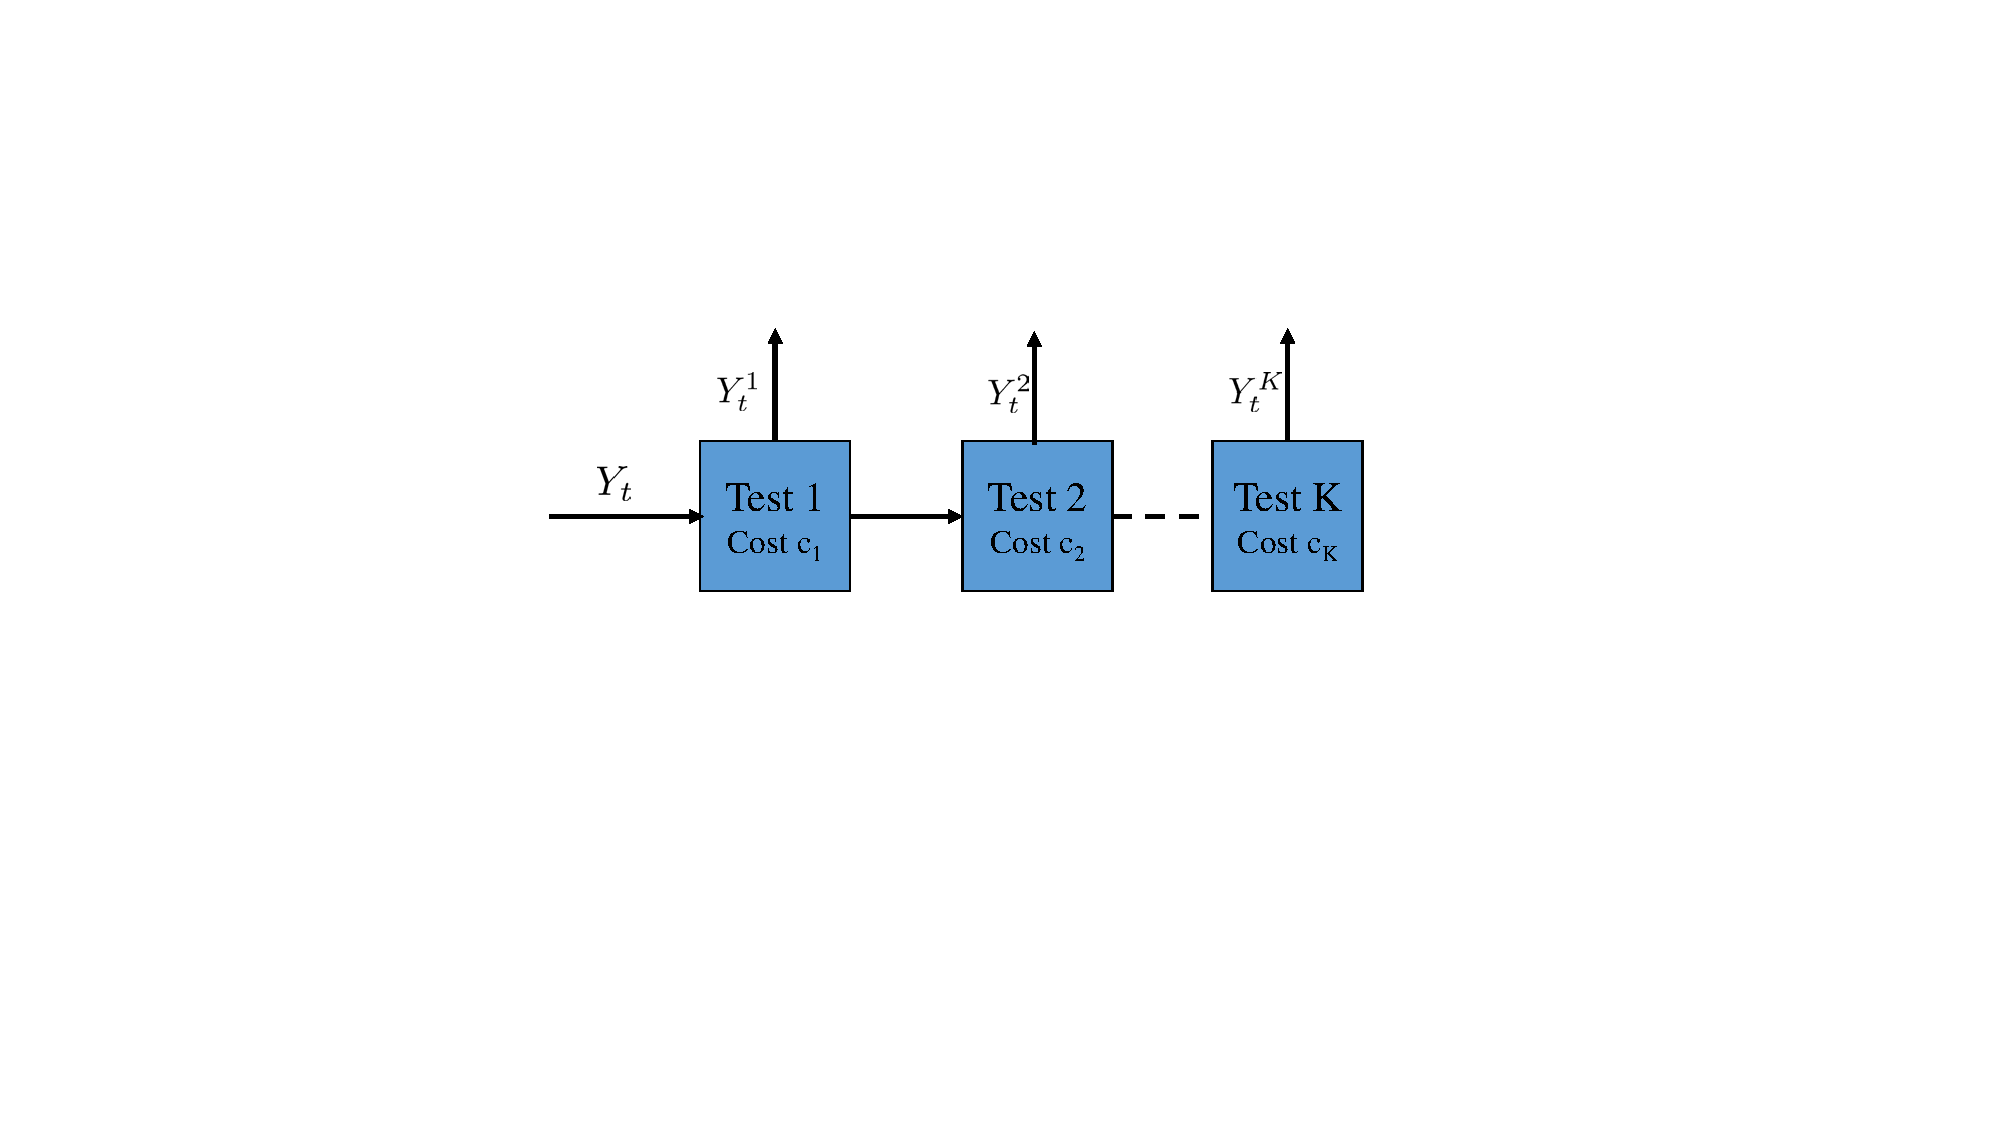
\includegraphics[scale=.6]{../Figures/cascade.pdf}
	\caption{Cascade of sensors
	}\label{wrap-fig:1}
	\vspace{-.5cm}
\end{wrapfigure} 

\if0
The prediction error rate of the $i^{th}$ sensor is denoted as $\gamma_i:=\Pr\{Y_t\neq \hat{Y}^k_t\}$. The learner incurs an extra cost of $c_k\geq 0$ to acquire output of sensor $k$ after acquiring output of sensor $k-1$. The sensor cascade is depicted in the adjacent figure. In this section we assume that the error rate does not depend on the  context, and the treatment with contextual information is given in the supplementary. 
\fi

%Let $H_t(k)$ denote the feedback observed in round $t$ from action $k$. Since we observe predictions of all the first $k$ senors by playing action $k$, we get   $H_t(k)=(\hat{Y}^1_t,\ldots,\hat{Y}^k_t)$.
%The loss incurred in each round is defined in terms of the prediction error and the total cost involved. When the learner selects action $k$, loss is the prediction error of sensor $k$ plus sum of the costs incurred along the path ($c_1,\ldots,c_k$). Let $L_t: \mathcal{A}\rightarrow \mathcal{R}_+$ denote the loss function in round $t$. Then,
%\begin{equation}
%L_t(k)=\mathbf{1}_{\{\hat{Y}^k_t\neq Y_t\}}+\sum_{j=1}^k c_j.
%\end{equation} 
We refer to the above setup as Sensor Acquisition Problem (SAP).
Based on the previous description, an instance of SAP is the tuple $\psi = (K,P,c)$, where $K\in \mathbb{N}$, $K\ge 2$,
$P$ is a distribution over $\{0,1\}^{K+1}$ and $c\in [0,\infty)^K$. 
 A policy $\pi$ on a $K$-sensor SAP problem
 is a sequence of maps, $(\pi_1, \pi_2, \cdots)$, where
 $\pi_t : \mathcal{H}_{t-1}\rightarrow [K]$ gives the action selected in round $t$
 given a history $h_{t-1}\in \mathcal{H}_{t-1}$ that consists of all actions and corresponding feedback observed before $t$. 
 Let $\Pi$ denote set of such policies. 
 For any $\pi \in \Pi$, we compare its performance to that of the single best action in hindsight 
 and define its expected regret as follows
\begin{equation}
R^\psi_T(\pi)= \mathbb{E}\left[\sum_{t=1}^T L_t(I_t)\right]-\min_{k\in A}\mathbb{E}\left[\sum_{t=1}^T L_t(k)\right],
\end{equation}
where $I_t$ denotes the action selected by $\pi_t$ in round $t$.

The goal of the learner is to learn a policy that minimizes the expected total loss, or, equivalently, to minimize the expected regret, i.e.,
\begin{equation}
\pi^*= \arg \min_{\pi \in \Pi } R^\psi_T(\pi).
\end{equation}

\noindent
{\bf Optimal action in hindsight: } For any $t$, we have 
\begin{equation}
\label{eqn:OptimalAction}
\mathbb{E}[L_t(k)]=\Pr\{Y_t\neq \hat{Y}^k_t\}+\sum_{j=1}^kc_j=\gamma_k +C_k\,,
\end{equation}
where $\gamma_k:=\Pr\{Y_t\neq \hat{Y}^k_t\}$ is the misclassification error rate of sensor $k$ and $C_k := c_1+\dots+c_k$ denotes the total cost for selecting the first $k$ sensors.
Since $c$ is assumed to be known, we will denote the dependence of the various quantities below
on $\gamma = (\gamma_1,\dots,\gamma_K)$ only.
Denote the expected cost of choosing action $k$ by $l_k(\gamma) = \gamma_k + C_k$. Let $k^* = \arg\min_{k\in [K]} l_k(\gamma)$ be the optimal action and let 
$\Delta_k(\gamma) = l_k(\gamma) - c^*(\gamma)$ be the expected excess cost of using action $k$.

The optimal policy is to play action $k^*$ in each round. If an action $i$ is played in any round then it adds $\Delta_i(\gamma)$ to the expected regret. 
Let $N_k(s)$ denote the number of times action $k$ 
is selected till time $s$, i.e., $N_k(s)=\sum_{t=1}^s \boldsymbol{1}_{\{I_t=k\}}$. 
Then the expected regret can be expressed as
\begin{eqnarray}
\label{eqn:ExpRegretGap}
<<<<<<< HEAD
R^\psi_T(\pi)&=& \sum_{k \in [K]}\mathbb{E}[N_k(T)]\Delta_k(\gamma)\,.
\end{eqnarray}
=======
R^\psi_T(\pi)&=& \sum_{k \in [K]}\mathbb{E}[N_k(T)]\Delta_k\,.
\end{eqnarray}\
\fi



\section{Weak Dominance}
\label{sec:Learnability}
%!TEX root =  main.tex
\vspace{-7pt}
Let $\TSA$ be the set of all stochastic, cascaded sensor acquisition problems. 
Thus, $\theta \in \TSA$ such that if $Y\sim \theta$ then $\gamma_k(\theta):=\Prob{Y\ne Y^k}$ 
is a decreasing sequence.
Given a subset $\Theta\subset \TSA$, we say that $\Theta$ is \emph{learnable} 
if there exists a learning algorithm $\Alg$ such that
for any $\theta\in \Theta$, the expected regret $\EE{ \Regret_n(\Alg,\theta) }$ 
of algorithm $\Alg$ on instance $\theta$ is sublinear.
A subset $\Theta$ is said to be a maximal learnable problem class if it is learnable and for any $\Theta'\subset \TSA$ superset
of $\Theta$, $\Theta'$ is not learnable.

\begin{defi}[Weak Dominance (WD)]
	An instance $\theta \in \TSA$  is said to satisfy the \emph{weak dominance,  property} if 
	for $i = a^*(\theta)$,
	\begin{align}
	\label{eq:wd} \rho = \min_{j > i} \frac{C_j - C_i}{\Prob{Y^i\ne Y^j}} \ge 1 %\forall j>i\,\,: \,\, C_j - C_i \ge \Prob{Y^i\ne Y^j}\,.
	\end{align}
We denote the set of all instances in $\TSA$ that satisfies this condition by $\TWD$.	
\end{defi}
\begin{thm}
The set $\TWD$ is essentially a maximal learnable set.
\end{thm}

Define a set $\mathcal{A}$ as follows:

\begin{align*}
\mathcal{A} =\bigg\{ i \in [K]:\, \forall j<i \,\,:\,\, C_i - C_j < \Prob{ Y^i \ne Y^j }\, \\
\mbox{  and  }\forall j>i \,\,:\,\, C_j - C_i \ge \Prob{ Y^i \ne Y^j }
\bigg \}\enspace.
\end{align*}

\begin{lem}
Let the WD conditions holds. Then the set $\mathcal{A}$ contains an optimal action, and it is a singleton set.
\end{lem}
\begin{proof}
It is clear that under WD property $\mathcal{A}$ contains an optimal action. We prove the second part by contradiction.  Assume that $i_1^\star, i_2^\star \in \mathcal{A}$ and $i_1^\star \neq i_2^\star$. WLOG, assume that $i_1^\star < i_2^*$. Since $i^\star_1 \in \mathcal{A}$, we have   $C_{j_1} - C_{i^\star_1} \ge \Prob{ Y^{i^\star_1} \ne Y^{j_1 }}$ for all $i_1^\star < j_1$. Also, since $i^\star_2 \in \mathcal{A}$, we have  $C_{i^\star_2} - C_{j_2 }< \Prob{ Y^{i^\star_2} \ne Y^{j_2} }$ for all $j_2 < i^\star_2$. 

Now, setting $j_1=i_2^\star$ and $j_2=i_1^\star$ above, we get    $C_{i_2^\star} - C_{i^\star_1} \ge \Prob{ Y^{i^\star_1} \ne Y^{i_2^\star}}$ and $C_{i^\star_2} - C_{i_1^\star }< \Prob{ Y^{i^\star_2} \ne Y^{i_1^\star} }$. Hence a a contradiction.
\end{proof}

%\begin{proof}
%\end{proof}
%We now relate WD to the optimality condition described in Eq.~\eqref{eqn:interp_opt}. WD can be viewed as a more stringent condition for optimal actions. For an action to be optimal we require that the marginal cost be larger than marginal \emph{absolute} error, namely, for all $j > i$, with $i = a^*(\theta)$:
%\begin{equation} \label{eqn:interp_WD}
%\underbrace{C_j - C_i}_{\text{Marginal Cost}} \geq \underbrace{ E \left [ \left | \ind{Y_t \ne Y_t^i} - \ind{Y_t \ne Y_t^j} \right | \right ]}_{\text{Marginal Absolute Error}}
%\end{equation}
%%The difference between marginal error in Eq.~\eqref{eqn:interp_opt} and
%where we have re-written $\Prob{Y^i\ne Y^j}$ as the marginal absolute error. We will show later that weak-dominant set is a maximal learnable set, namely, the set cannot be expanded while ensuring learnability.
%
%
%We propose the following action selector $\awd: M_1(\{0,1\}^K)  \to [K]$:
%\begin{defi}\label{def:awd}
%	For $P_S \in M_1(\{0,1\}^K) $ let $\awd(P_S)$ denote the smallest index $i\in [K]$ such that
%	\begin{subequations}
%		\begin{align}
%		\forall j<i \,\,:\,\, C_i - C_j < \Prob{ Y^i \ne Y^j }\,, \label{eq:wd1}\\ 
%		\forall j>i \,\,:\,\, C_j - C_i \ge \Prob{ Y^i \ne Y^j }\,, \label{eq:wd2}
%		\end{align}
%	\end{subequations}
%	where $C_i = c_1+\cdots + c_i$, $i\in [K]$ and $(Y^1,\dots,Y^K) \sim P_S$.
%	(If no such index exists, $\awd$ is undefined, i.e., $\awd$ is a partial function.)
%\end{defi}
%
%For any $\theta \in \TWD$ with $\theta = P_S\otimes P_{Y|S}$, $\awd(P_S)$ is well-defined and is essentially the only sound action selector map defined for all instances derived from the instances of $\TWD$. Further, the set $\TWD$ is essentially a maximal learnable set in the  $\mathrm{dom}(\awd)$, i.e., $\TWD$ is learnable but not uniformly learnable (see Appendix A for formal statements and proofs.).
%


%\section{Stochastic Multi-armed Bandits with Side Observations}
%\input{mab}
%
%\section{Regret Equivalence}
%\label{sec:Equiv}
%\vspace{-6pt}
%\input{equiv}

\vspace{-5pt}
\section{Algorithms}
\label{sec:Algo}
%!TEX root =  main.tex
%\subsection{Algorithm for Weak Dominance}
%\vspace{-4pt}
Define for any $i\neq j, \gamma_{ij}\doteq \Pr\{Y^i\neq Y^j\}$ and $\Delta_{ij}=C_j-C_i -\gamma_{ij}$. Our key insight for developing the algorithm is based on the fact that (see Def. 3),
under WD property, the set $\{i \in [K]: \min_{j> i}\Delta_{ij}\geq 0\}$ includes the optimal arm. We use this idea in Algorithm \ref{alg:UCB} to identify the optimal arm when an instance of USS satisfies WD. 

\begin{center}
\begin{minipage}{0.48\textwidth}
		\begin{algorithm}[H]
			\caption{Algorithm for USS with WD property} %ALG1}
			\label{alg:UCB}
			\begin{algorithmic}[1]
				\STATE Play action $K$ and observe $Y^1,\dots,Y^K$
				\STATE Set $\hgamma_{ij}(1) \set \one{Y^i\ne Y^j}$ for all $i< j$
				\STATE $n_i(1)\leftarrow \one{i=K} \; \forall i\in [K]$
				\FOR{$t=2,3,...$}
				\STATE $U_{ij}(t))\leftarrow\hgamma_{ij}(t-1) + \sqrt{\frac{1.5\log(t)}{n_j(t-1)}}$  for all $i< j$ \label{algo:UCB}
				\STATE $L_{ij}(t)\leftarrow\hgamma_{ij}(t-1) - \sqrt{\frac{1.5\log(t)}{n_j(t-1)}}$  for all $i< j$ \label{algo:LCB}
				\STATE $\hat{\Delta}_{ij}(t))\leftarrow C_j-C_i-L_{ij}(t)$ for all $i< j$
				\STATE $A_t \leftarrow \left \{i \in [K]:\displaystyle \min_{j> i}\hat{\Delta}_{ij}(t)\geq 0 \right\}$ \label{algo:sort}
				\STATE Set $\hat{I}_t\leftarrow \arg \min A_t\cup \{K\} $
				\STATE $B_t \leftarrow \left\{i>\hat{I}_t: C_i- C_{\hat{I}_t}-U_{\hat{I}_t i}^t \leq 0\right \}$
				\STATE $I_t\leftarrow \arg\min B_t\cup \{\hat{I}_t\}$
				\STATE Play $I_t$ and observe $Y^1,\dots,Y^{I_t}$.
				 \FOR {$i\in [I_t]$}
				\STATE $n_i(t) \set n_i(t-1)+1$\\
				 \STATE $\hgamma_{ij}(t) \set \left (1-\frac{1}{n_j(t)}\right )
				 \hgamma_{ij}(t-1) + \frac{1}{n_j(t)} \,\one{Y^j\ne Y^i}$ \\ $\forall i<j \leq I_t$ \label{algo:Update}
				\ENDFOR
				\ENDFOR
			\end{algorithmic}
		\end{algorithm}
	\end{minipage}
\end{center}

%
%Hence, we can express marginal error between sensors, $i,\,j$ as the difference between disagreements of sensors $i$ \& $1$, and sensors $j$ \& $1$. Under WD marginal error is only a lower bound on disagreement and so .   
%\todov{need to present a lower bound for reduction} 
%%when tests satisfy SD property, it can fail under WD (see Sec.~\ref{sec:Experiments}). 
%Our key insight is based on the fact that,
%%For any suboptimal arm $j < i^*$,  $C_{i^*}-C_j \leq \P\{Y^{i^*} \neq Y^j\}$ holds, and when the WD property holds, we further have $C_j -C_{i^*} \geq \P\{Y^i \neq Y^j\}$ for all $j>i^*$. 
%under WD, for a given set of the disagreement probabilities, for all $i \neq j$, the set $\{i \in [K-1]: C_j - C_i \geq \Pr\{Y^i \neq Y^j\} \mbox{ for all } j>i\}$ includes the optimal arm. We use this idea in Algorithm \ref{alg:UCB} to identify the optimal arm when an instance of USS satisfies WD. We will experimentally validate its performance on real datasets in the next section.
%The algorithm works as follows. It keeps track of $\hgamma^t_{ij}$ for all $i,j \in [K]$ and $i\neq j$ in each round, where $\hgamma_{ij}$ is an estimate of the probability $\P\{Y^i \neq Y^j\}$. In the first round, the algorithm plays arm $K$ and initializes its values. In each subsequent round, the algorithm computes the upper confidence value of $\hgamma^t_{ij}$ denoted as $U^t_{ij}$ (\ref{algo:UCB}) for all pairs $(i,j)$ and orders the arms: $i$ is considered better than arm $j$ if $C_j-C_i \geq U^t_{ij}$. Specifically, the algorithm plays an arm $i$ that satisfies $C_j-C_i \geq U^t_{ij}$ for all $j>i$ \ref{algo:sort}. If no such arm is found, then it plays arm $K$.  $n_j(t), j\in [K] $ counts the total number of observation of pairs $(Y^i, Y^j)$, for all $i<j$, till round $t$ and uses it to update the estimates $\hgamma_{ij}^t$ (\ref{algo:Update}).    % \rodos{Should we mention that due to lack of uniform learnability we do not present theoretical results here}
%=======
%The algorithm works as follows. It keeps track of $\hgamma^t_{ij}$ for all $i,j \in [K]$ and $i\neq j$ in each round, where $\hgamma_{ij}$ is an estimate of the probability $\P\{Y^i \neq Y^j\}$. In the first round, the algorithm plays arm $K$ and initializes its values. In each subsequent round, the algorithm computes the upper confidence value of $\hgamma^t_{ij}$ denoted as $U^t_{ij}$ (\ref{algo:UCB}) for all pairs $(i,j)$ and orders the arms: $i$ is considered better than arm $j$ if $C_j-C_i \geq U^t_{ij}$. Specifically, the algorithm plays an arm $i$ that satisfies $C_j-C_i \geq U^t_{ij}$ for all $j>i$ \ref{algo:sort}. If no such arm is found, then it plays arm $K$.  $n_j(t), j\in [K] $ counts the total number of observation of pairs $(Y^i, Y^j)$, for all $i<j$, till round $t$ and uses it to update the estimates $\hgamma_{ij}^t$ (\ref{algo:Update}).     \todov{Should we mention that due to lack of uniform learnability we do not present theoretical results here}

The algorithm works as follows. In each round, $t$, based on history, we keep track of estimates, $\hgamma_{ij}(t)$, of disagreements between sensor $i$ and sensor $j$.  %for all $i,j \in [K]$ and $i\neq j$ in each round, where $\hgamma_{ij}$ is an estimate of the probability $\P\{Y^i \neq Y^j\}$. 
In the first round, the algorithm plays arm $K$ and initializes its values. In each subsequent round, the algorithm computes the upper confidence value of $\hgamma_{ij}(t)$ denoted as $U_{ij}(t)$ (\ref{algo:UCB}) for all pairs $(i,j)$ and orders the arms: $i$ is considered better than arm $j$ if $C_j-C_i \geq U_{ij}(t)$. Specifically, the algorithm plays an arm $i$ that satisfies $C_j-C_i \geq U_{ij}(t)$ for all $j>i$ (\ref{algo:sort}). If no such arm is found, then it plays arm $K$.  $n_j(t), j\in [K] $ counts the total number of observation of pairs $(Y^i, Y^j)$, for all $i<j$, till round $t$ and uses it to update the estimates $\hgamma_{ij}(t)$ (\ref{algo:Update}).%However, note that due to the lack of uniform learnability under WD we cannot obtain a finite-time characterization and so omit these parallel results due to space limitations. 
%\vspace{-5pt}
\subsection{USS with Contextual Information } 
In this section we consider the case where contextual information associated with the instances are revealed in each round.  Let $\mathcal{X}\subset \mathbb{R}^D$ denote the set of contexts. For any cost vector $c$, the problem instance is specified by the pair $\bar{\theta}=(\bar{P},c)$, where $\bar{P}$ is a joint distribution over the set $\mathcal{X}\times\{0,1\}^{K+1}$. Specifically, $\bar{P}=P_{X}\otimes P_{Y|X}$, where $P_X$ is the distribution over $\mathcal{X}$ and $P_{Y|X}$ is the conditional distribution over $K+1$ binary vector given $X$. As earlier, we assume that $c$ is known and $\bar{P}$  is unknown, and we identify the problem instance $\bar{\theta}$ by $\bar{P}$. The learner-environment interaction is as follows: In  round $t=1,2,\ldots$, environment draws an independent sample  $Z_t=(X_t, Y_t, Y_t^1, \cdots,Y_t^K)$ distributed according to $\bar{P}$. The Learner observers $X_t$ and chooses index $I_t \in [K]$ upon which it further observers output of first $I_t$ sensors, i.e., $(Y_t^1, Y_t^2, \cdots, Y_t^{I_t})$. $Y_t$ is hidden and never observed.  Prediction accuracy of each sensor depends on the context. For sensor $k$ it is given by  $\bar{\gamma}: \mathcal{X}\rightarrow [0\;1]$ such that $\bar{\gamma}_k(x)=\bar{\gamma}_k(\bar{\theta},x)\doteq\Pr\{Y_t \neq Y | x\}$ for all $x\in \mathcal{X}$. We assume that sensors in the cascade are arranged in decreasing order of their prediction accuracy and this ordering is preserved for all contexts almost surely. Total cost incurred by the learner in round $t$ is thus $C_{I_t}+\ind{Y_t\neq Y_t^{I_t}|X_t}$. Let $\mu_k(x)\doteq \mu(\bar{\theta},x)=\mathbb{E}[C_k +\ind{Y_t\neq Y^{k}|x}]=C_k + \bar{\gamma}_k(x)$ denote the mean cost of action $k$ when the context is $x$. Let $\pi: \mathcal{X}\rightarrow [K]$ denote a policy that specifies action taken for each context, and let $\Pi$ denote the collection of all such policies. Given the values $\bar{\gamma}_k(\cdot)$ for all $k \in [K]$, let
$\pi^*\in \arg\min_{\pi \in \Pi} \mathbb{E}_{X \sim P_X}[C_{\pi(X)}+\bar{\gamma}_{\pi(X)}(X)]$ denote an optimal policy. The learner's goal is to learn a policy that competes with $\pi^*$. For any sequence of policies $\{\pi_t\}_{t\geq 1}$ where $\pi_t$ is the policy applied in round $t$, we define expected regret over time period $T$ as $\Regret_T(\bar{\theta})=\sum_{t=1}^T \mathbb{E}[\mu_{\pi_t(X)}(X)]- T\mathbb{E}[\mu_{\pi^*(X)}(X)]$


 For any $i\neq j$,  let $\bar{\gamma}_{ij}(x) \triangleq \Pr(Y^{i} \neq Y^{j}\mid x)$ denote probability that predictions of sensors $i$ and $j$ disagree on context $x$. We assume that this disagreement probability can be expressed as $\bar{\gamma}_{ij}(x)=\xi'f_{ij}(x)$, where $\xi \in \mathbb{R}^{d^\prime}$ is unknown parameter and $f_{ij}: \mathcal{X}\rightarrow \mathbb{R}^d$ is a fixed mapping that extracts the relevant features from each context that influence the disagreement rate of sensors $i,j$ .  More generally, we can assume that the disagreement probabilities can be expressed as a generalized linear model (GLM) as follows. For all $i\neq j$,  $\bar{\gamma}_{ij}(x)=F(\xi'f_{ij}(x))$, where $F(\cdot)$ is a non-negative real valued function.
 
 
 {Old Model:} when the log-odds ratio $\log \frac{\gamma_{ij}(x)}{1-\gamma_{ij}(x)}$ can be written as $\theta_{ij}'x$ for some unknown $\theta_{ij} \in \mathbb{R}^{d^\prime}$.
 
 \subsection{Algorithm}
\vspace{-5pt}
%  \todov{Should we mention that due to lack of uniform learnability we do not present theoretical results here}



\section{With Contextual Information}
%\section{Introduction}
%In many applications one has to make a trade-off between accuracy and cost. For example, in cost sensitive predictions, it is not only the accuracy of a sensor/test that matters, but also the cost of using it. Also, it may happen that one has to predict labels of instances for which ground-truth cannot be obtained. In such scenarios, feedback about correctness of sensor predictions is unknown. Such problems arise naturally in healthcare, security, crowd-sourcing, etc. In healthcare, the patients may not reveal outcome of a treatment due to privacy issues, hence effectiveness of the treatment cannot be known. In crowd-sourcing systems, the expertise levels of self-listed-agents (workers) are not known hence the quality of their work cannot be known. 
%
%In this work, we focus on the study of sensor selection problem where we do not have the advantage of knowing the ground-truth and hence cannot measure the error rates of the sensors. However, the goal is to still find the `best' sensor that gives smallest value of error plus cost. In such setup, it is natural to first use the sensor with lowest cost and then use the sensors with higher costs till sensor accuracy and cost is optimally traded. Such set of problems are referred to as Unsupervised Sequential Sensor (USS) acquisition problems \cite{hanawal2017unsupervised}. In the USS setup, it is assumed that the sensors form a cascade, i.e., they are ordered by their prediction efficiency-- the average prediction error decreases with every stage of the cascade. Though it is assumed that the sensor ordering is known and better sensors are associated with higher costs, the exact values of sensor errors are still unknown. The learner's goal is to find a sensor that has small value of  total prediction cost for a given task, which includes both the cost of acquiring the sensor outputs and the cost due to any incorrect prediction. Figure \ref{fig:USS} depicts the USS setup.
%%\begin{figure}[H]
%%	\centering
%%	\includegraphics[width=\linewidth]{figures/USS_Context.pdf}
%%	% % \caption{Unsupervised Sequential Sensor Acquisition}
%%	\caption{Cascaded Unsupervised Sequential Sensor Selection with Contextual Information. ${Y}_t^1 ,{Y}_t^2, \cdots , {Y}_t^K$, are sensor's outputs for context $x_t$ and $c_i$ denotes the acquiring cost of output for sensor $i$.}
%%	\label{fig:USS}
%%\end{figure}
%\vspace{-3mm}
%Each task is associated with side information or contextual information. For example, in healthcare the sensors could be various tests that need to be applied to ascertain existence of a condition in patients and each patient could represent a task through contextual information like, age, sex, height, etc. The optimal test applied on a task could depend on the task. Clearly, without the knowledge of the ground-truth one cannot find the optimal sensor as the sensor accuracies cannot be known. In the USS setup, the structure of the problem is exploited and when the weak dominance \cite{hanawal2017unsupervised} it is shown that  learning is possible. However, the goal in \cite{hanawal2017unsupervised} is to find the single best sensor to apply for each task and ignores any contextual information associated with them. Our goal in this work is to study how to use contextual information associated with each task to identify best test to apply on it.
%
%*** One more application: Deciding label of a input under unsupervised setting when multiple classifiers are given ***
%
%
%
%%~\\
%%\linebreak
%%\textbf{Our Contributions}\hspace{2mm}
%%We assume that prediction of each sensor is based on parameterized linear function of contexts (margins). Based on this, we have proposed different models in this report. In section 4, we propose a models to study the USS problem with side information and develop an algorithm that has sub-linear regret. We verify our result on synthetic \& real datasets. The learner observes only a noisy margin of the  selected sensors.
%%~\\
%%\linebreak
%%\textbf{Organization}\hspace{2mm} Section 3 introduces the unsupervised sensor selection problem with contextual case. Section 4 presents our margins based algorithm with weak regret bound and has experimentally verify on synthetic and real datasets. 
%%~\\
%%\linebreak
%%\textbf{Notation}\hspace{2mm}
%%$x_t \in \mathbb{R}^d$ represents context received at time $t$. Each context $x_t \sim \mathcal{D}$ where $\mathcal{D}$ is fixed and unknown distribution. The weighted $l_2$-norm associated with a positive definite matrix $A$ is defined by $\parallel x \parallel_A:= \sqrt{x^\top Ax}$. The set of actions is denoted by $[K]$. For each $a \in [K]$, $\theta_a^* $ denotes the fixed and unknown parameter associated with sensor $a$ and $\widehat{\theta}_t^a$ is an estimation of $\theta_a^\star$ using all the data collected till time $t-1$. We assumed, a fixed and known cost $c_a$ is associated with the sensor $a$. We assume $\parallel x_t \parallel_2 \leq L $ for all $t$ and $\parallel \theta_a^* \parallel_2\leq S$ for all $a\in [K]$  where both $S$ and $L$ are unknown. The sensor, arm and classifier are used interchangeably. The $\widehat{y}_t^a$ is the predicted margin value using the estimated classifier $\widehat{\theta}_t^a$ while $y_t^a$ is observed margin value when learner choose to play arm $a$ at round $t$.
%% The term sensors, tests and arms are used synonymously in this paper. Finally, $[n]:= \{1,2,\ldots,n\}$. In this report, the terms ``sensor'', ``test'' and ``classifier'' are synonymous.
%
%
%\section{Related Work}
%\cite{robbins1952mab}
%\subsection{Multi-Armed Bandits}
%\begin{description}
%	\item[Background of MAB]
%	\item[Sublinear Regret:] Expected v/s High Probability Regret 
%\end{description}
%
%%
%%\subsection{Different Reward Models for Contextual Bandits}
%%Brief details about Contextual Bandits.
%%\subsubsection{Linear Model}
%%With the development of modern technologies, contextual bandits have many applications in web based advertising and recommendation \cite{agarwal2009online, li2010contextual}. The most studied model in contextual bandits literature is the linear model \cite{auer2002using, dani2008stochastic, chu2011contextual, rusmevichientong2010linearly, abbasi2011improved}. The linear bandit model with side observation is also studied by \cite{valko2014spectral}. 
%%
%%\subsubsection{Genralized Linear Model}
%%Recently, \citep{filippi2010parametric, li2017provable, jun2017scalable} study the stochastic generalized linear models (GLM) in the contextual bandit setting which shows show $\sqrt{d}$ improvement over linear models. Linear, logistic and probit regression serve as three important special cases of GLM. 
%%\subsubsection{Nonlinear  Model}
%%Kernalized Model~\cite{Valko:2013:FAK:3023638.3023705}
%	
	
%\section{Problem Setting}
When the contextual information is available, the problem of the unsupervised, stochastic, cascaded sensor selection can be specified by a sequence $(X_t,Y_t, (Y_t^a)_{a \in [K]})$ of iid random variables, where $K$ is the number of sensors, $X_t \in \mathcal{X} \subset \mathcal{R}^\prime$ is the context at time $t$, $Y_t$ is the associated label and $Y_t^a$ is label predicted by sensor $a \in [K]$. The $K(>1)$ sensors are known to be ordered from least accurate to most accurate, i.e., expected error for a context $x$, $\gamma_a(x) := \Pr\{Y \neq Y^a|X=x\}$ of sensor $a$ is a decreasing function of $a$. As the setting considered is unsupervised, we do not have any knowledge about expected error $\gamma_a(x)$ except for their ordering which is assumed to remain the same for all contexts. Hence, given a context $x$, we need to make some assumptions for optimally choosing best option. 

For a given context, the total cost for selecting sensor $i$ is $C_i + \gamma_i(x)$, where $C_i=c_1 + \cdots + c_{i}$. The goal of the learner is to select an action that has smallest total cost (henceforth simply referred as cost) for a given context. For a given sequence of contexts $\{x_t\}_1^n$, we evaluate the learning performance a policy/algorithm that selects action $I_t:=I_t(x_t)$ in round $t$ in terms of the regret defined as follows:  
\vspace{-.1cm}
\begin{align}
\label{equ:lin_regret}
R_n = \sum_{t=1}^n\left(C_{I_t} + \gamma_{I_t}(x_t) - (C_{i^\star_t} +\gamma_{i^\star_t}(x_t))\right)
\end{align}
where 	$i_t^\star= \argmin_i(C_i + \alpha\gamma_i(x_t))$. The goal of the learner is to learn a policy that has lowest sub-linear regret, i.e., $R_n/n \rightarrow 0$ as $n \rightarrow \infty$ 
means that the learner in the long run collects almost as much reward on expectation as when  the optimal action is known. 

%Here $\mathbb{P}\{\bar{y}^i \neq \bar{y}^j|x\}$ represents the disagreement probability between observed labels of sensor $i$ and $j$ for a context $x$. \textcolor{blue}{Via an estimate of the probabilities sandwiched between costs and expected errors, one selects the arm to use.}


\subsection{Some Definitions}
%\textcolor{red}{Change notations and make these consistent with other part of report.}
Let $\Theta_{SA}$ be the set of all stochastic, cascaded sensor acquisition problems.
%Thus,  $\theta \in \Theta_{SA}$ such that if $Y \sim \theta$ then $\gamma_k(\theta) := \mathbb{P}(Y \neq Y^k)$ is a decreasing sequence. 
%Given a subset $\Theta \subset \Theta_{SA}$ , we say that $\Theta$ is learnable if there exists a learning algorithm $A$ such that for any  $\theta \in \Theta$, the expected regret $\mathbb{E}[\mathcal{R}_n(A, \theta)]$ of algorithm $A$ on instance $\theta$ is sublinear. A subset $\Theta$ is said to be a maximal learnable problem class if it is learnable and for any $\Theta^\prime \subset \Theta_{SA}$ super-set of $\Theta$, $\Theta^\prime$ is not learnable. We define two special learnable problem classes: Strong Dominance (SD) and Weak Dominance (WD), $\Theta_{SD} \subset \Theta_{WD}$ , where the regularity properties of the instances in  $\Theta_{SD}$ are more intuitive, while $\Theta_{WD}$ can be seen as a maximal extension of  $\Theta_{SD}$ .
%\begin{defi}[Strong Dominance (SD)] An problem instance $\theta \in \Theta_{SA}$ is said to satisfy the strong dominance property for all contexts if a sensor predicts correctly then all the sensors in the subsequent stages of the cascade also predict correctly, i.e., for any $i \in [K]$,
%	\begin{align} \label{equ:SD}
%Y^i = Y \Rightarrow  Y^{i+1} = Y \Rightarrow \cdots \Rightarrow Y^K = Y
%	\end{align}
%	almost surely (a.s.) where $(X, Y, Y^1, \cdots , Y^K) \sim P_\theta$.
%\end{defi} 
%
%\begin{defi} [Weak Dominance (WD) without context] An instance $\theta \subset \Theta_{SA}$ is said to satisfy the weak dominance property if the best action is $i^\star = a^\star(\theta)$. Then	
%	\begin{align} \label{equ:WD}
%	\forall j \in [K], \, j > i^\star : C_j - C_{i^\star} \geq \alpha\mathbb{P}(Y^{I} \neq Y^j)
%	\end{align}
	
	%\subsection{Strong Dominance and Weak Dominance property in Contextual Case}
	%	For any context $x \in \mathcal{X}$, the cost of selecting the $i$-th sensors in USS setting is  defined as $C_i + \alpha\gamma_i(x_t)$ where $C_i = c_1 + c_2 + \cdots + c_i$ with given positive $\{c_i\}_1^K$ and given $\alpha>0$. Let $\gamma_i(x):= \Pr\{\hat{Y}_i \neq y | X=x\}$ denote the error rate of sensor $i$ for context $x$ with label $y$. 
	%	% .0and $c_i$ represents cost of using sensor $i$.
	%	Let $i^\star(x)$ denote the best sensor for input $x_t$, i.e., 
	%	\begin{align}
	%	\label{equ:selection}
	%	i^\star(x) = \argmin_i(C_i + \alpha\gamma_i(x))
	%	\end{align}
	
%\end{defi} 

\begin{defi}[Weak Dominance with Contextual Information (WDC)] An instance $\theta \subset \Theta_{SA}$ is said to satisfy the weak dominance with contextual information property if for any context $x$ 	for all $ j \in [K], \, j > i^\star(x) $
	\begin{align} \label{equ:WDC}
C_j - C_{i^\star(x)} \geq \alpha\mathbb{P}(Y^{i^\star(x)} \neq Y^j|X=x)
	\end{align}
\end{defi} 
where $i^\star(x)$ is the optimal action for context $x$.
%\begin{define}[Sensor's Disagreement Indicator (SDI)] For given context $x$, the disagreement between predicted labels of two sensors $i$ and $j$ defines using sensor's disagreement indicator as follows
%	\begin{align*} 
%	d_{ij}(x) = \bigg\{\begin{array}{ll}
%	1, & Y_i \neq Y_j \text{ for given } x \\
%	0, & \text{o/w } 
%	\end{array} 
%	\end{align*}
%	Above equation can be written as:
%	\begin{align} \label{equ:SDI}
%	d_{ij}(x) = \mathbbm{1}_{\left\{\bar{y}^i \neq \bar{y}^j|x\right\}}
%	\end{align}
%\end{define} 

\begin{defi}[Sub-Gaussian Random Variables]
	Let $(X_t)$ be  $\{\mathcal{F}_t\}$ adapted: $\{\mathcal{F}_t\}$ is an increasing sequence of sigma fields such that $X_t$ is $\mathcal{F}_t$-measurable with $\mathbb{E}[X_t | \mathcal{F}_{t-1}] = 0$. Then, $\{X_t\}$ is a Sub-Gaussian with parameter $R$ if there exits $R>0$  such that for all $t$ and $\lambda \in \mathcal{R}$ the following holds:
	\begin{equation}
	\label{equ:sub_gaussian}
	\mathbb{E}\left[e^{\lambda X_t}| \mathcal{F}_{t-1}\right] \leq e^{\lambda^2R^2/2}
	\end{equation}
\end{defi} 


%\begin{define}
%	A  random  variable  $X \in \mathbb{R}$  is  said  to  be  sub-Gaussian  with  variance  proxy  $\sigma^2$  if  $\mathbb{E}[X] = 0$ and its moment generating  function satisfies 
%	
%	\begin{equation}
%	\label{equ:sub_gaussian1}
%	\mathbb{E}\left[exp(\lambda X)\right]\leq exp\left(\frac{\lambda^2\sigma^2}{2}\right) \;\; \forall \lambda \in \mathbb{R}
%	\end{equation}
%\end{define}

%\subsection*{Useful Results}
%\begin{lem}[\cite{abbasi2011improved}.]
%	\label{oful}
%	Let $V_t^a = X_{t-1}^a(X_{t-1}^a)^\top + \lambda I$ and $||\theta_a^\star||_2 \leq S$. For any $x \in \mathbb{R}^d$, $||x||_2 \leq L$ and $t \geq 1$, with probability at least $1-\delta$:
%	\begin{equation}
%	|x^\top(\widehat{\theta}_t^a - \theta_a^\star)|_{V_t^{-1}} \leq \beta_t^a||x||_{V_t^{-1}}
%	\end{equation}
%	where $\beta_t^a =  \lambda^{1/2}S + R\sqrt{2\log(1/\delta) + d\log(1 + C^aL/(\lambda d))}$ and $C^a$ is the number of times classifier $a$ is used till time $t$.
%\end{lem}
%%\begin{proof}
%%	Easily proves by using Theorem 3 of Abbasi et al.~\cite{abbasi2011improved}.
%%\end{proof}
%%
%%So, equation~\eqref{edq:disagreement} can be written using Lemma~\eqref{oful} as:
%%\begin{equation}
%%\label{estimate}
%%\widehat{y}_t^a = (\widehat{\theta}_t^a)^\top x_t +\beta_t^a ||x_t||_{(\overline{V}_t^a)^{-1}}
%%\end{equation}
%%
%%The Proposition 3 of Hanawal et al.~\cite{hanawal2017unsupervised} can be defined for contextual case as follows:
%%\begin{proposition} [ Proposition 3 of Hanawal et al.~\cite{hanawal2017unsupervised}]
%%	\label{pro:exp_err_prob}
%%	Let $\gamma_i(x)$ is the error rate of arm $i$ for given $x$, $\widehat{Y}_i$ is the label predicted by test/senor $i$ for given $x$   and $i < j$ then 
%%	\begin{align*}
%%	0 \leq \gamma_i(x) - \gamma_j(x) = \mathbb{P}\{\widehat{Y}_i \neq \widehat{Y}_j|x\} - 2\mathbb{P}\{\widehat{Y}_j \neq Y, \widehat{Y}_i = Y|x\} 
%%	% \text{\textcolor{red}{ Need to verify}}
%%	\end{align*}
%%\end{proposition}
%
%\begin{lem}
%	\label{lem:exp_err_prob}
%	\textbf{~\cite{hanawal2017unsupervised}[Prop. 3]}
%	Let $\gamma_i(x)$ is the error rate of arm $i$ for given $x$, $\widehat{Y}_i$ is the label predicted by test/senor $i$ for given $x$   and $i < j$ then 
%	\begin{align*}
%	0 \leq \gamma_i(x) - \gamma_j(x) = \mathbb{P}\{\widehat{Y}_i \neq \widehat{Y}_j|x\} - 2\mathbb{P}\{\widehat{Y}_j \neq Y, \widehat{Y}_i = Y|x\} 
%	% \text{\textcolor{red}{ Need to verify}}
%	\end{align*}
%\end{lem}
%\begin{proof}
%	\textcolor{red}{Similar to non-contextual case. Add it}
%\end{proof}
%~\\
%We can not evaluate expected loss $\gamma_i(x)$ but with {\it Strong Dominance} property, $\forall j>i, \, 2\mathbb{P}\{\widehat{Y}_j \neq Y, \widehat{Y}_i = Y|x\} = 0$ then equation in lemma~\ref{lem:exp_err_prob} can re-written as:
%\begin{align}
%\label{equ:sd_err}
%\gamma_i(x) - \gamma_j(x) = \mathbb{P}\{\widehat{Y}_i \neq \widehat{Y}_j|x\}
%\end{align} 
%
%\subsection{Modeling as Contextual Multi-Armed Bandit Problem}
%\subsubsection{Overview of Multi-Armed Bandit}
%\subsubsection{Multi-Armed Bandit with Side Information}
%First this problem is proposed by \cite{woodroofe1979one}.
%
%\vfill
	
	%\large{Unsupervised Cost Sensitive Predictions with Side Information}
\section{Disagreement based Model with Linear Assumption}
We assume that the disagreement between observed labels of sensors $i,j$ for a given context $x$ satisfies
%\begin{align}
%\label{equ:disagreement_prob}
%\mathbbm{1}_{\left\{\bar{y}^i \neq \bar{y}^j|x\right\}} = \mu({\phi_{ij}(x)^\top\theta^\star} ) + \epsilon_{i,j}
%%d_{ij}(x) = \mu({\phi_{ij}(x)^\top\theta^\star}) + \epsilon_{i,j}
%%d_{ij}(x) = \langle\,x_{i, j}, \theta^\star\rangle + \eta_{i,j} \text{ where } x_{i,j} = \Psi_{ij}(x)
%\end{align}
%where $\theta^\star$ is the true unknown coefficient vector, $\eta_{i,j}$ is assumed to be $R$-sub-Gaussian noise which statisfy equation \eqref{equ:sub_gaussian}  and $\phi_{ij}(x)$ is suitable feature map to get feature vector for sensor $i, j$ and given context $x$.
%
%The expected disagreement between predicated labels of two arms $i$ and $j$ is given by below equation: 
%\begin{align}
%\label{equ:exp_dis}
%\mathbb{E}\left[\mathbbm{1}_{\left\{\bar{y}^i \neq \bar{y}^j|x\right\}}\right] = \mu({\phi_{ij}(x)^\top\theta^\star})
%\end{align}
%We know the exception of indicator r.v. is given by
%\begin{align}
%\label{equ:exp_ind_pro}
%\mathbb{E}\left[\mathbbm{1}_{\left\{\bar{y}^i \neq \bar{y}^j|x\right\}}\right] = \mathbb{P}\left\{\bar{y}^i \neq \bar{y}^j|x\right\} 
%\end{align}
%From equation \eqref{equ:exp_dis},  and \eqref{equ:exp_ind_pro}, we can say that
\begin{align}
\mathbb{P}\left\{\widehat{Y}_i \neq \widehat{Y}_j|X=x\right\} = {\phi_{ij}(x)^\top\theta^\star}
\end{align}
where $\theta^\star \in \mathcal{R}^d$ is fixed but unknown and for all $i<j$, $\phi_{ij}: \mathcal{X} \rightarrow \mathcal{R}^d$ is a feature map. We assume that $d> d^\prime  $ and $||{\theta}^\star||_2 \le S$.

\subsection{Selection Criteria for Choosing Optimal sensor} The optimality of action (choosing sensor) can be captured in terms of marginal costs and marginal errors. In particular, for any context $x$ a sensor $i$ is optimal if for all $j > i$ the marginal increase in cost, $C_j - C_i$, is larger than the marginal decrease in error, $\gamma_i(x)-\gamma_j(x)$ i.e.,
\begin{align}
\label{equ:lin_cost_err}
%&C_j - C_i \ge \mathbb{E}[\mathbbm{1}_{\{Y \neq Y^i\}} - \mathbbm{1}_{\{Y \neq Y^j\}}]\nonumber \\
%&\Rightarrow 
\underbrace{C_j - C_i}_{\text{marginal cost}} \ge  \underbrace{\gamma_i(x)-\gamma_j(x)}_{\text{marginal error}}
\end{align}

Since $\gamma_i(x)$ is unknown for any $i$ and $x$, equation \eqref{equ:lin_cost_err} does not lead to an computational algorithm for sensor selection. So, we use the relation $\gamma_i(x)-\gamma_j(x)\leq\mathbb{P}\{Y^i\neq Y^j| X=x\}$ \cite{hanawal2017unsupervised}[Prop. 3] where $\widehat{Y}_i$ is label given for context $x$ by sensor $i$. Then using weak dominance condition of~\cite{hanawal2017unsupervised}[Def. 3], the weaker decision rule for selecting best sensor is given by

\begin{prop}
Assume that the weak dominance property holds. Let $i^\star(x)$ be the optimal action for context $x$.	Then,
\begin{align}
\label{equ:selection_label}
\forall j > i^\star (x),	C_j - C_{i^\star(x)} \ge \mathbb{P}\{Y^{i^\star(x)}\neq Y^j| X=x\}
\end{align}
\end{prop}
In the following we develop an algorithm that uses the above decision rule to select an optimal arm. The algorithm estimate the disagreement probabilities by comparing the predictions of the selected sensors. When the predictions of sensors $i,j$ are compared, the indicator value of the disagreements can be interpreted as a noisy version of their disagreement probability as give below

\[\mathbbm{1}_{\{Y^i \neq Y^j|X=x\}} = \mathbb{P}\{Y^i\neq Y^j|X=x\}+ \eta_{i,j}(x)\]
where $\eta_{i,j}(x)$ is a zero-mean bounded random variable and hence sub-Gaussian with some parameter $R$ (\colorbox{red}{Need to compute value of $R$}).
\subsection{Disagreement Model under Weak Dominance Property}
\begin{algorithm}[H]
	\caption{Linear Disagreement Model under Weak Dominance Property}
	\label{algo:linDM}
	\begin{algorithmic}[1]
		%   \Require
		\State \textbf{Input:} $\alpha > 0, R > 0, \lambda > 0, m \in \mathbb{N}, d \in \mathbb{N}, \delta \in (0,1)$
		\State $\overline{V}_0 = \lambda \mathrm{I}_d$, $M_0 = \ve{0}_d$ 
		\For{$t=1, 2, \ldots, m$} 
		\State Observe context, $x_t \in \mathbb{R}^d$
		\State Choose arm $I_t = K$
		\State Observe labels $\{\widehat{Y}_1^t, \widehat{Y}_2^t, \ldots, \widehat{Y}_{I_t}^t \}$; $\widehat{Y}_i^t \in \{0, 1\}$
		\State Construct feature vector using features of input $(x_t)$ and arm $i$ and $j$; $x_{i, j}^t \in \mathbb{R}^d$
		\State $\overline{V}_t = \overline{V}_{t-1} + \sum_{i=1}^{I_t-1}x_{i, I_t}^t (x_{i, I_t}^t)^\top$
		\State $M_t = M_{t-1} + \sum_{i=1}^{I_t-1}\mathbbm{1}_{\{\widehat{Y}_i^t \neq \widehat{Y}_{I_t}\}}x_{i, I_t}$ 
		\EndFor
		
		%  \State \\
		%   \State \textbf{Exploit-Explore Step}
		%   \For{$t=m+1, m+2, \ldots$}
		\For{$t=m+1, m+2, \ldots$}
		\State $\widehat{\theta}_t = \overline{V}_{t-1}^{-1}M_{t-1}$
		\State Observe context, $x_t$
		\State $\beta_t = R\sqrt{d\log\bigg(1 + \frac{tKL^2}{\lambda d}\bigg) + 2\log\bigg(\frac{1}{\delta}\bigg)} + \lambda^{1/2}S$
		\State \begin{align*}
	%	\label{eqn:SelectionCriteria}
\hspace{-.5cm}		\mathcal{A}_t =\bigg\{ i \in [K]:\, \forall j<i, \, C_i - C_j < \alpha\langle\,x_{i, j}^t, \widehat{\theta}_t\rangle -\, \beta_t ||x_{i,j}^t||_{\overline{V}_t^{-1}} \, \\
		\mbox{  and  }\forall j>i, \,C_j - C_i \ge\alpha\langle\,x_{i, j}^t, \widehat{\theta}_t\rangle -\, \beta_t ||x_{i,j}^t||_{\overline{V}_t^{-1}} 
		\bigg \}\enspace.
		\end{align*}
%		
%		
%		
%		\begin{equation}
%		\label{eqn:SelectionCriteria}
%		A_t= \{i \in [K]: \forall \;\; j \neq i  \;\;  C_j - C_i \geq \alpha\langle\,x_{i, j}^t, \widehat{\theta}_t\rangle -\, \beta_t ||x_{i,j}^t||_{\overline{V}_t^{-1}} \}\cup\{K\}
%			\end{equation}
		%   \textcolor{red}{LB or UB??? $->$ LB}
		\State If $\mathcal{A}_t \neq \emptyset$, set $I_t= \arg\min \mathcal{A}_t$. Else $I_t=K$.
		\State Observe labels $\{\widehat{Y}_1^t, \widehat{Y}_2^t, \ldots, \widehat{Y}_{I_t}^t \}$
		\State $\overline{V}_t = \overline{V}_{t-1} + \sum_{i=1}^{I_t-1}x_{i, I_t}^t (x_{i, I_t}^t)^\top$
		\State $M_t = M_{t-1} + \sum_{i=1}^{I_t-1}\mathbbm{1}_{\{\widehat{Y}_i^t \neq \widehat{Y}_{I_t}^t\}}x_{i, I_t}$
		\EndFor
		
	\end{algorithmic}
\end{algorithm}

\subsection{Regret Analysis of Disagreement Model}
\label{sec:dma_regret}
Regret analysis is similar to that for the OFUL algorithm given in paper~\cite{abbasi2011improved}.

\subsubsection{Important Lemmas and Theorems}
\label{sec:dma_regret_lemmas}
Some of the lemma derived using results from paper~\cite{abbasi2011improved, hanawal2017unsupervised}.
\begin{lem}
For any $i,j \in [K] $ and any context $x$ the following relations hold.
\begin{align}
\label{eqn:disagree1}
\gamma_i(x)-\gamma_j(x)& = \Pr\{Y^i \neq Y^j|X=x\}  \nonumber \\
&-2\Pr\{Y^i=Y, Y^j \neq Y|X=x\}.
\end{align}	
\begin{align}
\label{eqn:disagree2}
\gamma_i(x)-\gamma_j(x) =& -\Pr\{Y^i \neq Y^j|X=x\} \nonumber \\
&+2\Pr\{Y^i \neq Y, Y^j = Y|X=x\}.
\end{align}	
\end{lem}
		
\begin{lem}
	\label{lem:confidence}
	% \textbf{~\citep{abbasi2011improved}}  
	Let $\overline{V}_t = \sum_{s=1}^{t}\sum_{j=1}^{I_t-1}x_{j, I_t}^s(x_{j, I_t}^s)^\top + \overline{V}_0$ and $S_t = \sum_{s=1}^{t}\sum_{j=1}^{I_t-1}\eta_{j,I_t}^sx_{j, I_t}^s$. Then, for any $\delta > 0 $ with probability at least $1-\delta$, for all $t \geq 0$,
	\begin{align*}
	||S_t||_{\overline{V}_t^-}^2 \le 2R^2\log\bigg(\frac{det(\overline{V}_t)^{1/2}det(\overline{V}_0)^{-1/2}}{\delta}\bigg)
	\end{align*}
\end{lem}

\begin{lem}
	\label{lem:diff} 
	Let $\overline{V}_t$ be as defined in Lemma~\ref{lem:confidence} and  let $\overline{V}_0 =\lambda I_d$. Assume that $||\theta^\star||_2 \le S$. Then, for any $\delta > 0$ with probability at least $1-\delta$, for all $t \ge 0$ and $ x^t$,
	\begin{align*}
	|\langle\,x_{i, j}^t, \theta^\star\rangle - \langle\,x_{i, j}^t, \widehat{\theta}_t\rangle|\le \beta_t||x_{i,j}^t||_{\overline{V}^-_t}
	\end{align*}
	where $\beta_t = R\sqrt{d\log\bigg(1 + \frac{tKL^2}{\lambda d}\bigg) + 2\log\bigg(\frac{1}{\delta}\bigg)} + \lambda^{1/2}S$ 
	% $\beta_t \le R \sqrt{2\log\bigg(\frac{det(\overline{V}_t)^{1/2}det(\lambda I_d)^{-1/2}}{\delta}\bigg)} + \lambda^{1/2}S $
\end{lem}

\begin{lem}
	\label{lem:x_norm}
	For any $1 \le i < j \le K$, $\{x_{i,j}^s\}_{s=1}^\infty$ be a sequence in $\mathbb{R}^d$, $V$ is a $d \times d$ positive definite matrix and define $\overline{V}_t = V + \sum_{s=1}^{t}\sum_{j=1}^{I_t-1}x_{j, I_t}^s(x_{j, I_t}^s)^\top$. Then, we have that 
	\begin{align*}
	\sum_{t=1}^n \min\{1, ||x_{i,j}^s||_{\overline{V}_{t-1}^-}^2\} \le 2\log\frac{det(\overline{V}_n)}{det(V)}
	\end{align*}
	Further if $||x_{i,j}^s||_2 \le L$ for all $t$ and $\lambda_{min}(V) \ge \max\{1, L^2\}$, then
	\begin{align*}
	\log\frac{det(\overline{V}_n)}{det(V)} \le \sum_{t=1}^n ||x_{i,j}^s||_{\overline{V}_{t-1}^-}^2 \le 2\log\frac{det(\overline{V}_n)}{det(V)}
	\end{align*}
\end{lem}

% \begin{lem}
% \label{lem:det_trc}
% (Determinant-Trace Inequality) Suppose $X_1, X_2, \vdots, X_t \in \mathbb{R}_d$ and for any $1 \le s \le t$, $||X_s||_2 \le L$. Let $\overline{V}_t = \lambda I_d + \sum_{s=1}^{t}X_sX_S^\top$, for some $\lambda > 0$. Then
% \begin{align*}
% det(\overline{V}_t) \le (\lambda + tL^2/d)^2
% \end{align*}
% \end{lem}

\begin{lem}
	\label{lem:det_trc}
	% (Extension of Lemma~\ref{lem:det_trc}) 
	% If algorithm receives on average $A_{I_t}$ samples instead of one sample $X_s$ in one round and
	(Determinant-Trace Inequality) Suppose $K$ is total number of sensors/tests, for any $1 \le s \le t$ and $1 \le j < I_t \le K$, $||x_{j, I_t}^s||_2 \le L$ where $x_{j, I_t}^s \in \mathbb{R}^d$. Let $\overline{V}_t = \lambda I_d + \sum_{s=1}^{t}\sum_{j=1}^{I_t-1}x_{j, I_t}^s(x_{j, I_t}^s)^\top$, for some $\lambda > 0$. Then  
	\begin{align*}
	% det(\overline{V}_t) \le (\lambda + A_{I_t}tL^2/d)^2 \le (\lambda + KtL^2/d)^2
	det(\overline{V}_t) \le (\lambda + tKL^2/d)^2
	\end{align*}
	\begin{proof} By inequality of arithmetic and geometric means,
		\begin{align*}
		det(\overline{V}_t) \le (trace(\overline{V}_t)/d)^d
		\end{align*}
		As the trace of matrix is a linear mapping i.e. $trace(A+B) = trace(A) + trace(B)$, hence
		\begin{align*}
		trace(\overline{V}_t) &= trace(\lambda I_d) + \sum_{s=1}^{t}\sum_{j=1}^{I_t-1}trace(x_{j, I_t}^s(x_{j, I_t}^s)^\top) \\
		&= d\lambda + \sum_{s=1}^{t}\sum_{j=1}^{I_t-1}||x_{j, I_t}^s||_2^2 \\
		&= d\lambda +\sum_{j=1}^{I_t-1}\sum_{s=1}^{t}||x_{j, I_t}^s||_2^2 \\
		% &\le d\lambda + \sum_{j=1}^{I_t-1}tL^2\\
		% &\le d\lambda + t\sum_{j=1}^{I_t-1}||x_{j, I_t}^s||_2^2 \\
		\Rightarrow trace(\overline{V}_t) &\le d\lambda + tKL^2 \text{ as } I_t \le K
		\end{align*}
		Using this result, we get
		\begin{align*}
		det(\overline{V}_t) &\le (trace(\overline{V}_t)/d)^d \\
		&\le \big((\lambda d + tKL^2)/d\big)^d \\
		\Rightarrow det(\overline{V}_t) &\le (\lambda + tKL^2/d)^d
		\end{align*}
	\end{proof}
\end{lem}

\begin{lem}
	\label{lem:tight_det_trc}
	Assume same as in lem~\ref{lem:det_trc},  let $A_{I_t} = \frac{1}{t}\sum_{s=1}^{t}I_s$ where $I_s$ is the optimal sensor/test chosen by algorithm for data instance $x_s$. 
	\begin{align*}
	det(\overline{V}_t) \le (\lambda + tA_{I_t}L^2/d)^2
	\end{align*}
	
	\begin{proof}
		As we know, 
		\begin{align*}
		trace(\overline{V}_t) &= d\lambda +\sum_{j=1}^{I_t-1}\sum_{s=1}^{t}||x_{j, I_t}^s||_2^2  \\
		&\le d\lambda + tA_{I_t}L^2 \text{ where $A_{I_t} \le K$}
		\end{align*}
		By inequality of arithmetic and geometric means,
		\begin{align*}
		det(\overline{V}_t) &\le (trace(\overline{V}_t)/d)^d  \\
		\Rightarrow det(\overline{V}_t) &\le (\lambda + tA_{I_t}L^2/d)^2
		\end{align*}
	\end{proof}
\end{lem}

%\begin{lem}
%	\label{lem:je_reg}
%	Let $1/T$ is the probability of choosing $a_t$ for $t \in [T]$ from a sequence of $\{a_1, a_2, \cdots , a_T\}$. Then
%	\begin{align*}
%	\sum_{t=1}^T a_t \le \sqrt{T\sum_{t=1}^T a_t^2}
%	\end{align*}
%	\begin{proof}
%		(By Jensen's Inequality) If $f$ is a convex function then
%		\begin{align*}
%		f(\mathbb{E}[X]) \le  \mathbb{E}[f(X)]
%		\end{align*}
%		Let $f$ is a square function i.e. $f(x) = x^2$ and $X$ is a r.v. which represents the chosen $a_i$. Then
%		\begin{align*}
%		f(\mathbb{E}[X]) &= \bigg( \sum_{t=1}^T \frac{a_t}{T}\bigg)^2
%		\le \mathbb{E}[f(X)] 
%		\le \frac{1}{T}\bigg( \sum_{t=1}^T a_t^2\bigg) \\
%		\Rightarrow \sum_{t=1}^T a_t &\le \sqrt{T\sum_{t=1}^T a_t^2}
%		\end{align*}
%	\end{proof}
%\end{lem}


%\subsubsection{Cost and Expected Error Relationship}
%To reflect the optimistic principle of algorithm, Arm $I_t$ has lowest cost i.e. $C_{I_t} + \alpha\gamma_{I_t}(x_t)$. Then following lemma will hold:
%\begin{lem}
%	\label{lem:cost_err}
%	If arm $I_t$ is best arm chosen by the algorithm and $\overline{V}_0 = \lambda I_d$ then
%	\begin{align*}
%	\text{For } j > I_t; \text{ } C_{I_t} - C_j \leq -\alpha\langle\,x_{i,j}^t,\widehat{\theta}_t\rangle + \alpha \beta_t||x_{i,j}^t||_{\overline{V}^-} 
%	\end{align*}
%\end{lem}
%\begin{proof} From optimal criteria, smallest $I_t$ is best arm if 
%	\begin{align*}
%	C_j - C_{I_t} \geq  \alpha[\gamma_{I_t}(x_t) - \gamma_j(x_t)]
%	\end{align*}
%	We have
%	\begin{align*}
%	C_{I_t} - C_j &\leq  -\alpha(\gamma_{I_t}(x_t) - \gamma_j(x_t)]) \\
%	&\leq  -\alpha\mathbb{P}\{\widehat{Y}_i^t \neq \widehat{Y}_j^t|x_t\}  \nonumber \\
%	&\leq  -\alpha(\langle\,x_{i,j}^t,\widehat{\theta}_t\rangle -  \beta_t||x_{i,j}^t||_{\overline{V}^-}) \mbox{ By Lemma } 4.2\\
%	\Rightarrow C_{I_t} - C_j &\leq -\alpha\langle\,x_{i,j}^t,\widehat{\theta}_t\rangle + \alpha \beta_t||x_{i,j}^t||_{\overline{V}^-} 
%	\end{align*}
%\end{proof}

% \subsubsection{Cost-Expected Error Relationship}
% \label{sec:ra_}


\subsubsection{Instantaneous Regret}
\label{sec:ra_ir}
The instantaneous regret of algorithm is the regret incurred for any time t. 

\begin{thm}
	\label{thm:ir}[\colorbox{red}{This proof is not complete}]
	The instantaneous regret $r_t$ of algorithm with probability at least $1-\delta$ is:
	\begin{align*}
	r_t \le 2\alpha \beta_t ||x_{I_t, i^\star}^t||_{\overline{V}^-}
	\end{align*}
\end{thm}
\begin{proof}
	\begin{align*}
	r_t &= C_{I_t} + \alpha\gamma_{I_t}(x_t) - \argmin_i(C_i + \alpha\gamma_i(x_t)) \\
	&= C_{I_t} + \alpha\gamma_{I_t}(x_t) - (C_{i^\star_t} + \alpha\gamma_{i^\star_t}(x_t)) \\
	&= C_{I_t} - C_{i^\star_t} + \alpha(\gamma_{I_t}(x_t) - \gamma_{i^\star_t}(x_t)) \\
%	&\le C_{I_t} - C_{i^\star} + \alpha\mathbb{P}\{\widehat{Y}_{I_t}^t \neq \widehat{Y}_{i^\star}^t|x_t\} 
	% &\le C_{I_t} - C_{i^\star} + \alpha x_{t, a}^\top \theta^* \text{ using linear assumption}
	\end{align*}
where $i_t^\star$ is the best arm in round $t$. Two possibilities arises: $I_t > i_t^\star$ or $I_t \leq i_t^\star$. First consider the case $i^\star_t > I_t$. From the previous lemma we have
	\begin{align*}
	r_t &= C_{I_t} - C_{i^\star_t} + \alpha(\gamma_{I_t}(x_t) - \gamma_{i^\star_t}(x_t)) \\
	&\le  -\alpha\langle\,x_{I_i,i^\star}^t,\widehat{\theta}_t\rangle + \alpha \beta_t||x_{I_t, i^\star}^t||_{\overline{V}^-_t}  + \\
	& \;\;\;\; \alpha \Pr\{Y^{I_t}\neq Y^{i^\star_t}|X=x_t\} \mbox{     from (\ref{eqn:SelectionCriteria}) and (\ref{eqn:disagree1})}\\ 
	&= \alpha(\langle\,x_{I_i,i^\star}^t, \theta^\star-\widehat{\theta}_t\rangle  + \alpha \beta_t||x_{I_t, i^\star}^t||_{\overline{V}^-_t} \\
	&\le \alpha \beta_t||x_{I_t, i^\star}^t||_{\overline{V}^-_t} + \alpha \beta_t||x_{I_t, i^\star}^t||_{\overline{V}^-_t} \text{ from lemma~\ref{lem:diff}}\\
	&= 2\alpha \beta_t||x_{I_t, i^\star}^t||_{\overline{V}^-_t}
	\end{align*}
Now consider the case 	$i^\star_t \leq I_t$. Using Equation \ref{eqn:disagree2} we get
\begin{align*}
r_t &= C_{I_t} - C_{i^\star_t} + \alpha(\gamma_{I_t}(x_t) - \gamma_{i^\star_t}(x_t)) \\
&=C_{I_t} - C_{i^\star_t} - \alpha\Pr\{Y^{I_t}_t \neq Y^{i^\star_t}_t| X=x_t\} + \\
& \;\;\; 2\alpha\Pr\{Y_{t}^{I_t} \neq Y_t,Y^{ i^\star_t}_t =Y_t| X=x_t \}\\
& \le \alpha \langle\,x_{I_t,i^\star_t},\widehat{\theta}_t\rangle + \alpha \beta_t||x_{I_t, i^\star}^t||_{\overline{V}^-_t} -\alpha\langle\,x_{I_i,i^\star}^t, \theta^\star\rangle +\\
& \;\;\;\; 2\alpha\Pr\{Y_{t}^{I_t} \neq Y_t,Y^{ i^\star_t}_t =Y_t| X=x_t \}\\
& \le \alpha \langle\,x_{I_t,i^\star_t},\widehat{\theta}_t-\theta^\star\rangle + \alpha \beta_t||x_{I_t, i^\star}^t||_{\overline{V}^-_t} + \\
& \;\;\;\; 2\alpha\Pr\{Y_{t}^{I_t} \neq Y_t,Y^{ i^\star_t}_t =Y_t| X=x_t \}\\
& \le 2\alpha \beta_t||x_{I_t, i^\star}^t||_{\overline{V}^-_t} +  2\alpha\Pr\{Y_{t}^{I_t} \neq Y_t,Y^{ i^\star_t}_t =Y_t| X=x_t \}\\
& =(??) 2\alpha \beta_t||x_{I_t, i^\star}^t||_{\overline{V}^-_t} +  2\alpha\Pr\{I_t \neq  i^\star_t | X=x_t \}\
\end{align*}
	\colorbox{red}{
		How to get rid of the second term here?}
\end{proof}


\subsubsection{Cumulative Regret}
\label{sec:ra_cr}
\begin{thm}
	\label{thm:cr}
	The cumulative regret $R_T$ of disagreement model for time horizon $T$ with probability at least $1-\delta$ is:
	\begin{align*}
	R_T \le 2\alpha \bigg( R\sqrt{d\log\bigg(1 + \frac{KTL^2}{\lambda d}\bigg) + 2\log\bigg(\frac{1}{\delta}\bigg)} + \lambda^{1/2}S\bigg) \sqrt{2Td\log\bigg(1 + \frac{KTL^2}{\lambda d}\bigg)}
	\end{align*}
\end{thm}

\begin{proof}
	\begin{align*}
	R_T &= \sum_{t=1}^T r_t \\
	&\le \sqrt{T\sum_{t=1}^T r_t^2} \\
	&\le \sqrt{T\sum_{t=1}^T \left[2\alpha \beta_t||x_{i,j}^t||_{\overline{V}^-}\right]^2} \text{ from theorem~\ref{thm:ir}} \\
	& \text{ As $\beta_t \le \beta_T$ because $\beta_t$ is not decreasing with $t$ (by definition of $\beta_t$)} \\
	&\le 2\alpha \beta_T \sqrt{T\sum_{t=1}^T \left[||x_{i,j}^t||_{\overline{V}^-}\right]^2}  \\
	% \text{ $\beta_t$ is not decreasing with $t$} \\
	&\le 2\alpha \beta_T \sqrt{T * 2\log\bigg(\frac{det(\overline{V})}{det(\lambda I_d)}\bigg)} \text{ from lemma~\ref{lem:x_norm}} \\
	% &\le 2\alpha \beta_T \sqrt{2T\log\bigg(1 + \frac{tKL^2}{\lambda d}\bigg)^d} \text{ from lemma~\ref{lem:det_trc}} \\
	&\le 2\alpha \beta_T \sqrt{2Td\log\bigg(1 + \frac{tKL^2}{\lambda d}\bigg)}  \text{ from lemma~\ref{lem:det_trc}} \\
	&\le 2\alpha \beta_T \sqrt{2Td\log\bigg(1 + \frac{KTL^2}{\lambda d}\bigg)}   \text{ as } t \le T \\
	& \text{Now using value of $\beta_T$ and lemma~\ref{lem:det_trc}} \\
	% &\le 2\alpha \bigg(R \sqrt{2\log\bigg(\frac{det(\overline{V}_T)^{1/2}det(\lambda I_d)^{-1/2}}{\delta}\bigg)} + \lambda^{1/2}S\bigg) \sqrt{2Td\log\bigg(1 + \frac{TL^2}{\lambda d}\bigg)} \\
	% &  \text{ Using estimate for determinate of matrix i.e. $det(\overline{V}_t)$ from lemma~\ref{lem:det_trc}}\\
	&\le 2\alpha \bigg( R\sqrt{d\log\bigg(1 + \frac{KTL^2}{\lambda d}\bigg) + 2\log\bigg(\frac{1}{\delta}\bigg)} + \lambda^{1/2}S\bigg) \\
	& \sqrt{2Td\log\bigg(1 + \frac{KTL^2}{\lambda d}\bigg)}
	\end{align*}
\end{proof}
\vspace{-0.8cm}
%\subsubsection{Commutative Regret - Special Case}
%\label{sec:ra_crs}
%\begin{corollary}
%	If  $A_{I_t} = \frac{1}{t}\sum_{s=1}^{t}I_s$ is estimated then using lemma~\ref{lem:tight_det_trc} and theorem~\ref{thm:cr}, the commutative regret $R_T$ of disagreement model for time horizon $T$ with probability at least $1-\delta$ is:
%	\begin{align*}
%	R_T \le 2\alpha \bigg( R\sqrt{d\log\bigg(1 + \frac{A_{I_t}TL^2}{\lambda d}\bigg) + 2\log\bigg(\frac{1}{\delta}\bigg)} + \lambda^{1/2}S\bigg) \sqrt{2Td\log\bigg(1 + \frac{A_{I_t}TL^2}{\lambda d}\bigg)}
%	\end{align*}
%\end{corollary}
%
%\subsection{Difficulties with Linear Disagreement Model} 
%The samples for which two sensors disagree are linearly inseparable. Before using above model, one should come up with suitable feature map $\Psi_{ij}(x)$  for given sensors $i, j$ and context $x$. 
%\\
%\textcolor{red}{Add figures to show above claim, if possible, prove it}



%\section{Experiments}
%\label{sec:Experiments}
%\input{exp}

%\vspace{-10pt}
%\section{Conclusions}
%\label{sec:Conclu}
%%\input{conclude}
%\vspace{-10pt}
%The paper describes a novel approach for unsupervised sensor selection. These types of problems arise in a number of healthcare and security applications. In these applications we have a collection of tests that are typically organized in a hierarchical architecture wherein test results are acquired in a sequential fashion. The goal is to identify the best balance between accuracy \& test-costs. The main challenge in these applications is that ground-truth annotated examples are unavailable and it is often difficult to acquire them in-situ. We proposed a novel approach for sensor selection based on a novel notion of weak and strong dominance properties. We showed that weak dominance condition is maximal in that violation of this condition leads to loss of learnability. Our experiments demonstrate that weak dominance does hold in practice for real datasets and typically for these datasets, unsupervised selection can be as effective as a supervised (bandit) setting. 
%
%\section*{Acknowledgment}
%\label{sec:Ack}
%M. K. Hanawal would like to thank support from INSPIRE faculty award (IFA-14/ENG-73, 16DSTINS002) from Department of Science and Technology, Government of India and SEED grant (16IRCCSG010) from IIT Bombay.
%\bibliographystyle{biblio}
\bibliographystyle{IEEEtran}
\bibliography{ref}


%\newpage
%\section*{\large Supplementary material for the paper titled Unsupervised Sequential Sensor Acquisition}
%\hrulefill \hrulefill
%\hrulefill
%\input{append}



\end{document}




